\documentclass{article}
\usepackage[round]{natbib}

\usepackage{fullpage}
\usepackage{listings}
\usepackage{url}
\usepackage{authblk}
\usepackage{graphicx}
\usepackage{color}
\usepackage{hyperref}
\usepackage{amsmath,amssymb}

\setlength{\parindent}{0pt}
\setlength{\parskip}{1em}

\lstset{language=Python}

% local definitions
\newcommand{\comment}[1]{{\textcolor{red}{Comment: #1}}}

\newenvironment{response}%
  {\list{}{\leftmargin=0.5in\rightmargin=0.5in\color{blue}}\item[]}%
  {\endlist}

\usepackage{lipsum}

\begin{document}

May 27, 2021

GENETICS-2021-304236
Can we distinguish modes of selective interactions using linkage disequilibrium?

Dear Dr. Ragsdale:

Your manuscript has been evaluated by two reviewers.  I agree with the
assessment of the reviewers of that this has the potential to be an important
contribution but that it is not there yet.  Your manuscript would need to be
revised substantially, including conducting additional analysis, to be
acceptable for publication in GENETICS.  Please understand that incremental
changes will not be sufficient.  If you intend to resubmit, please let the
editorial office know approximately how long you expect to need for revisions.
Upon resubmission, please include a detailed response to the reviewers'
comments and to the concerns listed above; it will likely be sent out for
review.  I am hopeful you will be willing to do these revisions as I am excited
about the potential of your manuscript.

\begin{response}
    Dear Dr. Agrawal,

    Thank you for the opportunity to revise this manuscript for consideration
    in Genetics and your patience in completing the revisions. I appreciate
    the careful reading and detailed comments that you and each reviewer have
    made, and I believe that these suggestions have substantially improved the
    paper. Below, my responses to each comment are indented and in blue.

    I'd first like to highlight a few of the more substantial changes:
    \begin{itemize}
        \item The addition of a large suite of numerical validations against
            individual-based simulations, as well as a handful of forward
            simulations to demonstrate the effects of many linked loci on diversity
            statistics
        \item A new Figure 1 that provides some intuition for the two-locus
            sampling distribution and its summaries (contrasted with the SFS
            and its summaries)
        \item Extended numerical analyses, in particular for patterns of LD under
            dominance models
        \item Partitioning LD by allele-frequency binning -- in particular, the
            result of increased LD among missense mutations within conserved
            domains is driven by common variants above $\approx 10\%$
            (I expand on this below)
    \end{itemize}

    \noindent
    Sincerely,\\
    Aaron Ragsdale
\end{response}

The manuscript has a theoretical and empirical component and each needs
revision.  The reviewers have each made a number of comments that should be
addressed and I will summarize the main ones from my perspective.

Theoretical Section: I agree with the reviewers that there is value in your
numerical approach to two-locus sampling distribution. This comment from
Reviewer 2 captures my sentiment: ``the first part of the manuscript does not
seem to fully capitalize on the potential that these new numerical approaches
offer to build quantitative in the extremely large space of models that is
explored.'' Here are what I view as the most important ways the theory section
of the ms should be developed:

1) The numerical approach is based on some approximations but there is no
testing of how well these approximations hold. I agree with both reviewers that
there should be some level of testing (via comparison to forward simulations)
to show how well these approximations work and, when they fail, what kind of
biases they cause.

\begin{response}
    The Supporting Material now includes validation using discrete
    forward simulation. The forward simulations are individual based
    Wright-Fisher simulations, with implementation details in the Supporting
    Material. These comparisons show that the numerical approach introduced in
    this paper is accurate for the weak to moderate recombination and selection
    strengths studied in this paper ($\rho, \gamma \lesssim 30$).
    Most simulations only tracked the allele frequencies at the two loci,
    neglecting the background selection-like effects,
    although I also ran a small number of simulations of larger genomic
    regions that allowed many mutations to segregate at once. These are included
    in the Supporting Information.
\end{response}

2) There should be some theoretical results presented for using allele
frequency thresholds or allele frequency bins. LD patterns may differ between
rare versus common variants and, further, this would allow comparison to the
manuscript by Good cited in the current ms (but not very meaningfully
discussed) as raised by Reviewer 2. More generally, to extent to which the
patterns you report in Figures 1-3 were driven by rare or common variants. For
example, I found myself wondering whether the effects of the population size
changes you reported may be different for LD among rare variants vs LD among
common variants. (Further, empirical data may be filtered by frequency for
other reasons; see below.)

\begin{response}
    This is an important point, and I agree that describing expectations of LD
    for different frequency bins and thresholds will be useful for interpreting
    the theoretical and empirical results presented here. From the two-locus
    sampling distribution, it is straightforward to compute LD based on
    arbitrary observed allele count conditions, and I now include figures showing
    expected LD for varying conditions for the same selection scenarios I had
    highlighted before.
\end{response}

3) Both reviewers pointed out that selection occurs at more than two sites and
that pairwise LD could be affected by selection at other loci. That seems an
important caveat that should be stated and ideally tested.

\begin{response}
    Thank you for the suggestion. I now include this caveat at the beginning
    of the results. I also include a some simulations of large regions with
    many selected loci to give a sense of the bias caused by selection at other
    loci than the focal pair.
\end{response}

4) I did not look at the scripts you made available but I would encourage you
to make them as user-friendly as possible. This ms has the potential to make a
bigger impact if it is easy for empirical (not just theoretical!) population
geneticists to use your scripts.

\begin{response}
    I am happy to make all scripts public, and I have tried to keep
    an organized an documented/commented repository of all scripts used in the
    analysis here (\url{https://www.github.com/apragsdale/two_locus_selection.git}).
    Additionally, the numerical methods are implemented, documented, and tested
    within the \emph{moments} software (which includes single-locus SFS and
    multi-population LD methods, documentation at \url{https://moments.readthedocs.io/}),
    which I and other developers actively maintain.
\end{response}

Empirical Section: The analysis of the human data builds up the original
analysis of Sohail et al. by focusing primarily on intragenic LD patterns. The
results are presented in a manner to contrast different mutation classes (e.g.,
synonymous, missense, LOFs) with the implication being that a difference in LD
among classes is due to differences in the nature of selection among these site
types. However, there are several key concerns:

5) Allele frequencies. The LD patterns reported using the full spectrum of
allele frequencies. However, the allele frequency spectrum will be different
among these mutational classes, which is an important confounding effect that
should be considered. Reviewer 1 suggests allele frequency matching. In
addition to allele frequency matching, there is good reason to consider
different allele frequency classes separately if you are interested in making
inferences about selection because a substantial fraction of missense mutations
are likely to be effectively neutral (and some might even experience balancing
selection); low frequency missense variants are likely to be in more heavily
enriched for deleterious vs. effectively neutral variants compared to
intermediate or high frequency variants. For this reason, I would like to see
an analysis using only rare variants or, even better, to consider multiple
different allele frequency categories separately (e.g., $p < 0.02$, $0.02 \leq
p \leq 0.1$, $p > 0.1$). Consider your striking pattern for within-domain LD
for missense mutations. My interpretation of what that pattern might indicate
is quite different if it is driven entirely by intermediate frequency variants
rather than by rare variants. Further, examining LD patterns for different
allele frequency bins could dovetail nicely with suggestions made for the
theoretical section.

\begin{response}
    Thank you for this suggestions.
    Previously I had matched synonymous and missense mutations only for distances,
    and not frequency. I now also partition mutations by allele frequencies
    (rare: $p\lesssim 0.02$, uncommon: $0.02\lesssim p \lesssim 0.1$, and common).
    From this, the opposing patterns of increased or decreased LD between missense
    mutations within vs outside of conserved domains is predominantly driven by
    pairs of common variants. The unconditioned statistic \(\sigma_d^1\) is
    already dominated by common variants, so I don't think this result is too
    surprising.

    In interpreting this result, this suggests to me that there is something
    more interesting going on than the explanation that common missense
    mutations are simply effectively neutral. Assuming synonymous mutations are
    effectively neutral (this is of course not always the case, although common
    synonymous mutations would be neutral by the same argument, and we don't
    see a difference in Tajima's D for syn variation within vs outside of domains),
    we still observe increased LD of missense mutations over that of synonymous
    mutations. If missense mutations at these common frequencies were entirely
    neutral, we'd expect their levels of LD
    to be roughly equal to those of synonymous mutations.

    Background selection also appears to have minimal effects on signed LD between
    neutral mutations (Supp Figures 7--10), so I lean toward the explanation that
    some form of direct selection/interactions on those missense mutations (or at
    least a subset of them) is driving this signal. More careful analysis is needed
    to say anything definitively, which I have left for future work.
\end{response}

6) Distances. The average pairwise distance will be lower for mutational
classes that are more abundant. Presumably LOFs are much less abundant than
synonymous or missense mutations so I suspect that the average pairwise
distance between LOFs is larger than for other two types (which probably differ
from one another). Though this won't affect the sign of LD it is obviously
expected to affect the magnitude.

\begin{response}
    In the previous version of the manuscript, I had considered average LD for
    pairs of mutations outside of domains weighted to match the distances between
    mutations observed inside domains. I repeated that analysis here and placed
    more emphasis on comparing pairs at matching distances (see Supp Fig 26 for a
    comparison of density of pairs in differnece classes at given distances).
    For the LOFs, that is a good point, although how few LOF pairs exist within
    the same gene makes further subsetting of LOFs difficult.
    I now include this caveat in the Discussion.
\end{response}

Some other comments of my own.

7) I don't like the title as I don't believe it reflects the value of your
contributions. (I like the work presented in this ms but I do not think this ms
does a particularly strong job of carefully considering or answering the
question posed by the title.)

\begin{response}
    I have changed the title, and agree that the previous title wasn't a great
    fit. Now:
    ``A heterogeneous landscape of selection and epistasis  in
    protein-coding genes revealed by two-locus statistics''
\end{response}

8) See the recent PNAS paper from Denis Roze (2021), which has analytical
results showing the effect of dominance on LD. He shows positive LD if $h < 0.25$
and negative LD otherwise.

\begin{response}
    Thank you for bringing this paper to my attention, which I had not seen
    previously. I now include a direct comparison to Denis Roze's paper, shown
    in Figure 4. That result of positive LD when $h<0.25$ appears to only hold
    for very strongly selected mutations. For weak to moderate selection,
    this threshold can change, and some parameter values give LD less than zero
    for all $0 \leq h \leq 1$. I now show these comparisons and results and discuss
    them in the main text.
\end{response}

9) The legend of Figure 4 reads, ``Loss-of-function mutations are defined as
stop and start gains and losses and other nonsense mutations of high impact.''
Please explicitly specify what ``other nonsense mutations of high impact'' means
in the Methods; I couldn't find anything explicit.

\begin{response}
    This is now clarified in the Methods.
\end{response}

10) Line 340-345: You are of course correct when averaging over all allele
frequencies. However, migration generate positive LD among derived variants
when conditioning on those variants being rare (see Sandler et al. 2021, Fig
S3). (An example of how LD patterns can be sensitive to allele frequency
class!)

\begin{response}
    Thanks for this clarification, and I have updated the Discussion to
    make this point clearer.
\end{response}

11) Line 350: The comment about Sandler et al is misleading from my
perspective. The gene flow simulations were not intended to quantitatively
mimic the data (the intention was to simply show a qualitative match, i.e.,
positive LD); it is easy to make LD from gene flow go up or down in magnitude
by tweaking the magnitude and nature of gene flow in the simulation. (Moreover,
that figure was removed for other reasons from the revised version of that ms.)

\begin{response}
    My apologies for potentially misrepresenting the results from those simulations
    in Sandler et al -- that certainly wasn't my intention. I have removed these
    lines in this version of the manuscript, though I do think the observation is
    important that positive LD between synonymous mutations only extends over short
    distances (a few hundred base pairs). I have edited the Discussion about this point.
\end{response}

12) Line 350-360. The point about multinucleotide mutations (MNMs) is
important. I would have liked to see more detail in the legend of Figure S8 of
what was actually done to produce this figure (i.e., enough of a methods
description that one could reproduce this). While the model fits reasonably
well, it implicates what seems like a very proportion of multinucleotide
mutation events. Is there any evidence to support this, perhaps from Icelandic
trio dataset? I am not suggesting you need to do a formal analysis (though it
would be great if you did) but you should comment on whether there is any
evidence that the estimated fraction of MNMs is realistic. (A personal note: I
think you are right to point out that MNMs make the ``null'' expectation to be
positive LD because MNMs are a biological reality. I take the same attitude to
population structure / gene flow. The question then becomes about the relative
importance of the two as the source of positive LD for neutral variants. I do
not claim to know with certainty the answer to that question but I am highly
skeptical that MNMs are sufficient to explain long range positive LD. To be
clear, I am not requiring you to convince me otherwise, but I will be impressed
if you can!)

\begin{response}
    I have extended the methods description for this analysis in the Supplement, as
    well as refined the inference to directy estimate the proportion of mutations
    that result in MNM events instead of simply fitting the probability that an
    \emph{observed} pair of mutations at a given distance were caused by a MNM event.
    
    In the previous version of the manuscript, I pointed out (though I think not too
    clearly) that the proportion of pairs of mutations observed at a given distance
    that arose through a MNM event is different than the proportion of new mutation events
    that are single- vs multi-nucleotide mutations. The probability that a new
    mutation results in a MNM can be very small (much less than 1\%), but the proportion
    of mutation pairs we observe that were initially MNM events can be quite high
    (e.g., 5--10\%). I expand on this point in the Supplement.

    In fitting the MNM model to synonymous data, I infer that new mutations affect
    multiple nucleotides at relatively small rates ($\ll 1\%$). However, because of
    the scaling of the non-MNM two-locus sampling distribution in $\theta^2$ and
    the scaling of the MNM two-locus sampling distribution proportional to
    $\theta \cdot p_{MNM}$, up to $10\%$ of observed mutations at short distances may
    have arisen from MNM events. I expand on this in the Supplement.
\end{response}

Sincerely,

Aneil Agrawal\\
Associate Editor\\
GENETICS\\

\textbf{Reviewer \#1:}

The manuscript by Ragsdale examines two-locus sampling distributions with
arbitrary natural selection and complex demographies. In particular, the author
uses a numerical approach of moment closures to compute the expected number of
two-locus haplotype counts under complex evolutionary models. Previously,
two-locus sampling distributions were only available for neutral models. Models
including selection were only accessible via forward simulations or assuming
selected variants are independent of one another. As such, this paper addresses
an important problem in the field, providing a much-needed solution.

Further, these two-locus models provide the opportunity to study patterns of
epistasis, which has not received as much attention in the empirical population
genetics literature. Thus, I predict this work will be foundational for future
theoretical and empirical studies.

While I am very positive about the paper as a whole and the potential of the
methods, I have a number of major comments that should be addressed prior to
publication:

1) In the Results and Discussion, it is important to emphasize that these
predictions are for the LD between 2 loci that could be in LD with each other,
but are not linked to other selected loci. In real genomes, the pair of
selected loci could be linked to other nearby selected variants that could have
an effect on the LD of the focal pair. As studying a region with many
deleterious mutations would be even bigger undertaking than that presented
here, I do not think that this problem needs to be solved in this manuscript.
Rather, adding a simple caveat to the paper should suffice.

\begin{response}
    I agree this is an important point, and also think that fully accounting
    for many linked selected mutations is beyond the scope of this paper. I have
    included a caveat when introducing numerical methods.

    I also now include a few forward-in-time individual-based simulations
    of large regions with high rates of selected mutations, to get an idea of the
    magnitude of distortion that can occur due to background selection, associative
    overdominance, and linked purifying selection. These are included in the Supplement.
\end{response}

2) It would be good if some of the predictions for the behavior of LD
statistics in complex models could be verified through forward in time
simulations (using SLiM or something similar). This isn't necessary for all
models (because that is the point of the numerical methods to avoid lots of
simulations), but I think it would add rigor to this work to show that at least
for some models, the predictions match up to the simulations.

\begin{response}
    I have now included a simulation of a region allowing many simultaneous
    deleterious mutations (with only Hill-Robertson interference, that is,
    no epistasis), for additive ($h=0.5$) and recessive ($h=0, 0.1$) mutations.
    The goals of these larger simulations were to explore the effects of multiple
    linked selected loci.

    In addition to these simulation, I ran a large suite of discrete simulations
    tracking haplotype frequencies for pairs of loci under range of epistatic
    and dominance interaction scenarios, comparing the resulting two-locus
    sampling distribution. These are shown in the Supplement and online
    documentation of moments and this manuscript, and show good agreement between
    simulations (in the absense of BGS) and the numerical approach introduced here.
\end{response}

3) Analysis of empirical data (Fig 4 and Fig 5): Missense and variants within
protein domains seem to be in more positive LD than those not within protein
domains or synonymous SNPs. This is an interesting and potentially important
result. It does not appear that the different types of variants were matched
for allele frequency. Missense and synonymous SNPs have very different allele
frequency distributions, with the former having more rare variants. It is
well-known that allele frequencies can influence LD statistics (see for
example, vanLiere \& Rosenberg (2008 TPB); Hedrick (1987 Genetics); Eberle et
al. (2006 PLoS Genetics)). Further, the fact that Table S4 shows that Tajima's
D differs among these different types of variants further supports the notion
that the allele frequencies inside protein domains differ from those outside.
Thus, I'm concerned that the differences in LD patterns can be simply driven by
differences in allele frequency, rather than differences in LD driven by
epistasis or compensatory mutations. Matching on allele frequency when
computing the LD statistics would alleviate this problem.

\begin{response}
    Thank you for these suggestions. While I had matched pairs of mutations based
    on distances, I had not matched by allele frequences. As mentioned above,
    I now condition on both alleles being rare, uncommon, or common and compare
    LD across these categories.
    From this, the opposing signals of increased/decreased
    LD between missense mutations within/outside of domains is driven by
    mutations with frequencies greater than $0.1$. The agreement between
    high-frequency-conditioned and unconditioned $\sigma_d^1$ is unsurprising,
    since $\sigma_d^1$ is dominated by mutations at common frequencies (while
    $r$ and $r^2$ are more sensitive to rare variants).
    I now include a much larger set of conditioned LD comparisons (in the
    Supplement, Tables S6--S11 and Figures S20-S24).
\end{response}

4) Related to point 3 above, when analyzing the empirical data, are the
synonymous and missense variants from the same protein domains? Or, are there
some domains that may only have synonymous variants and others that have only
missense variants? In the latter scenario, the synonymous variants would not be
as good of a control for the missense variants because they are in different
genomic regions. While I think it's great that Tajima's D was compared for
variants within and outside of protein domains, I wonder about other
properties, such as recombination rate or strength of background selection
(maybe quantified by the McVicker B- value). If domains have different
recombination rates than do the coding regions outside of domains, then this
could lead to LD patterns appearing different.

\begin{response}
    I agree that there are many potentially confounding factors when making comparisons
    between different genomic regions (even within the same gene), and even when
    comparing classes of mutations within the same region. I now include
    these caveats in the Discussion.
    
    To your point about genes and domains containing different numbers of synonymous
    vs missense mutations, I tested the correlation between those numbers at both
    the gene and the domain level (Supp Figures 24 and 25). At the gene level (which
    are larger regions that contain more mutations overall), there is a fairly strong
    correlation between numbers of missense and synonymous mutations ($r=0.86$).
    This correlation is somewhat weaker at the domain level,
    as these are smaller regions ($r=0.57$). Because there are already relatively few
    mutations within domains overall, leading to larger measurement noise, I chose not
    to reduce the total number of compared pairs of mutations even further.
\end{response}

Minor comments:

1) Abstract, line 11: Maybe say, ``distorting allele frequency trajectories and
creating correlations between pairs of mutations''.

\begin{response}
    Thank you for the suggestion.
\end{response}

2) Introduction, line 28: It would be good to provide some references in the
first paragraph about deleterious mutations and negative selection, how they
affect neutral regions. Further, references should be provided when saying that
something is ``empirically documented''.

\begin{response}
    Thank you for the suggestions. I have added references in the first paragraph
    of the Introduction as suggested.
\end{response}

3) The terms ``synergistic'' and ``antagonistic'' epistasis are used extensively
throughout. It would be good to provide a more clear definition of these terms
early on in the manuscript and how they are used here for describing
deleterious mutations.

\begin{response}
    Thank you for the suggestion. In the first paragraph of the Empirical observations
    section, where the term ``synergistic'' epistasis is first used, I attempted
    to make the definition a bit more clear. I do the same for both synergistic and
    antagonistic epistasis when introducing the epistasis models in the results.
\end{response}

4) Caption of Figure 1: I believe that the signs of the synergistic and
antagonistic epistasis are reversed. Given the definition in Methods, shouldn't
epsilon be $>0$ for synergistic epistasis as more deleterious mutations have
lower fitness than predicted under multiplicative models? Then, epsilon would
be $<0$ for antagonistic epistasis.

\begin{response}
    Thank you for catching this error, and I'm sorry if it caused any confusion.
    Caption fixed.
\end{response}

5) Figures 1-2: I think it would be good to highlight that these plots show the
expected values of these LD statistics for the given models.

\begin{response}
    I have updated the figure captions to clarify that
    expectations of LD that are being plotted.
\end{response}

6) Line 142: When mentioning that mean LD can extend over 100kb, I think it
would be good to also put this more in terms of human-like parameters, as the
physical distance over which LD is expected to extend under these models would
depend on the recombination rate.

\begin{response}
    Thank you for the suggestion. I have updated this section to be more explicit
    in this regard.
\end{response}

7) Line 146: Cite some references if saying that the effect of epistasis on LD
is widely studied.

\begin{response}
    With the rearrangement of the text, this line has been removed.
\end{response}

8) Supplementary Figure 1: I think it would be instructive to move this to the
main text to show a more intuitive depiction of the 2-locus sampling
distribution.

\begin{response}
    A new Figure 1 in this version hopefully provides a more intuitive depiction
    of the two-locus sampling distribution and its summaries (with direct comparison
    to the SFS and some of its summaries). Thank for you this suggestion, and I hope
    the new figure is helpful in introducing these statistics.
\end{response}

9) Lines 285-289: These lines seem at odds with what Garcia \& Lohmueller
reported. They found that interference interactions are likely common among
nonsynonymous mutations and that nonsynonymous variants have more LD than
synonymous ones.

\begin{response}
    Thanks for pointing this out, and this is now clarified in the Discussion.
\end{response}

10) Line 417: Yun Song has done some theory on expectations of r2 in Song \&
Song (2007, TPB). This work should be cited here.

\begin{response}
    Thank you for the suggestion. Song and Song, 2007 is now commented on here.
\end{response}

11) Line 548: More detail should be given in this section about how the
analysis of non-steady state demography was done here.

\begin{response}
    This is now expanded on in the Methods.
\end{response}



\textbf{Reviewer \#2:}

In this manuscript, the author investigates expected patterns of linkage
disequilibrium (LD) between two genetic loci under a range of evolutionary
models. In the first part of the manuscript, the author extends a previous
numerical approach by Ragsdale and Gravel (2019) to calculate the expected
sampling distribution of two-locus haplotypes under any selection model. The
author uses this approach to investigate the effects of Hill-Robertson
interference, epistasis, dominance, and changing demography on patterns of LD,
and then uses these insights to analyze and interpret patterns of excess
linkage between non synonymous variants within conserved elements.

In general, I think this is a very interesting and important topic, and I think
there are many interesting observations made by the author. I struggle however
with the manuscript overall, for two reasons. First, while I generally strongly
agree that numerical approaches to estimating population genetic quantities in
more computationally tractable ways than whole-population whole-genome
simulations, the first part of the manuscript does not seem to fully capitalize
on the potential that these new numerical approaches offer to build
quantitative in the extremely large space of models that is explored. Second, I
am not sure that this two-locus intuition can be directly translated to
interpret patterns of human genetic diversity, given that human genomes may be
experiencing selection at a large number of linked loci, which may lead to
behaviors that are not seen in the two-locus model alone. Finally, I have a
technical concern about the limitations of the moment closure approach and
wonder whether these technical limitations force the conclusion about epistasis
made in the last part of the manuscript. I explain my concerns in detail below.

Major comments:

1) As far as I can tell, the calculations in the SI are correct under the
approximations made, but there is very little discussion of the importance of
the approximations made and the limitations these impose for interpreting data.
Specifically, the condition that $r$ and $s$ are order $1/N_e$ and that $n \ll
N_e$ implies that $ns \ll 1$. This means that this approach is unable to
accurately capture the statistics of mutations segregating at frequencies of
order $1/Ns$ or larger. I find this both broadly and specifically concerning.
Specifically, Good (2020) bioRxiv [cited within the discussion] has
demonstrated that it is precisely these mutations that show an excess of LD
that resembles the effects of antagonistic epistases, even in purely additive
models, which is not seen here. This concern is also directly related to the
finding that antagonistic epistasis may be responsible for unusually high LD
within genes -- it is unclear to me whether negative selection alone may be
responsible for these patterns.

\begin{response}
    I appreciate the concern about accuracy of the numerical methods, and I
    have added extensive validations against simulations for the cases
    of additivity, synergistic epistasis, antagonistic epistasis, and recessive
    mutations. For the parameter values considered here
    ($\rho, |\gamma| \approx 0 - 30$), we find very good agreement between simulation
    and numerical solutions. The condition that $r$ and $s$ are of order $1/N_e$
    is standard in the diffusion approximation, allowing us to neglect terms
    of order $s^2$, $rs$, $s/N_e$, etc. In practice, diffusion methods still
    provide reasonably accurate results for larger selection and recombination
    values, and only break down for very strong
    selection beyond the parameter ranges I considered here
    (see, e.g., Krukov and Gravel, bioRxiv 2021)

    I don't exactly follow the conclusion, that ``This means that this approach
    is unable to accurately capture the statistics of mutations segregating at
    frequencies of order $1/Ns$ or larger.'' The condition that $ns\ll 1$ is only
    violated for extremely strong selection (say, $|s| \gtrsim 0.01$, as sample sizes
    that I consider here are not too large). But that strength of selection is beyond
    the results presented in this paper.

    I have expanded on the parameter ranges that this method is applicable for
    and point to simulation results showing accuracy over this range of parameters.
\end{response}

2) More broadly, without more detailed exploration of the parameter space of
the models considered and without more work to interpret quanitatively at which
frequencies different behaviors will occur as a function of the parameters, it
is difficult to interpret the generalizability of the results quoted here. Note
that this is especially a concern when the results are used to shape
qualitative insights about the patterns seen in genomes. It would be important
to describe the theoretical reasoning behind the choice of specific values of
parameters the simulations, and why the author believes they tile the space of
important behaviors of a two locus model.

\begin{response}
    I agree that it is difficult to make more definitive claims about the
    causes of variation in patterns of LD seen in the data without a more
    detailed exploration of the relevant parameter space. Ideally, this would
    come in the form of likelihood-based inference of the joint effects of 
    selection and interactions, as well as validation against models of BGS.
    I comment on this in the Discussion but leave it to future work.

    I have expanded the theoretical/numerical results to consider additional
    parameters and the dependence on frequency conditioning, though this still
    falls short of a complete exploration of parameter space. I focused primarily
    on selection strengths in the range $\gamma\approx -1$ to $-10$, as these
    selection strengths show the largest effects of interference without 
    epistasis, including for dominance. The very large space of possible selection
    models makes it difficult to fully tile this space. Nonetheless, I
    believe that the results presented in the main text and the expanded results
    in the Supplement are useful for building intuition about the behavior or
    two-locus statistics under different interaction models.
    I have also edited the Discussion to include these caveats and
    point to future work in these directions.
\end{response}

3) On a related note, given the restriction that $n \ll N$, many of these
results should be directly comparable to the recent analytical results from
Good (2020) bioRxiv on expected patterns of LD in a two-locus model. I think
that using the rationale developed by that and similar studies would really
make it possible to capitalize on the ability to rapidly calculate LD in a
broader range of contexts.

\begin{response}
    This is a good suggestion, I spent quite a bit of time trying to implement
    the analytical results from Good (2020). I was unable to make much
    progress in such a comparison. For the most part, I was able to replicate
    the results in Figures 3 and 4 in that paper (e.g., see below, though there
    are noticeable differences between the written formulae and the plots in
    Figure 3 in Good).
    But to compare the analytical results in Good (2020) directly
    to the numerical approximations
    here, we need to make use of the finite sample estimators (Appendix G in Good).
    Unfortunately, I was unable to obtain sensical results implementing the
    formulae in Appendix G, and there may be one (or more) typos in Appendix G
    that make a direct comparison impossible without rederiving those results.

    I did not include this figure in my revision here, because I could not
    faithfully recreate the results presented in Figure 3 in Good 2020.
\end{response}

\begin{figure}[h!]
    \centering
    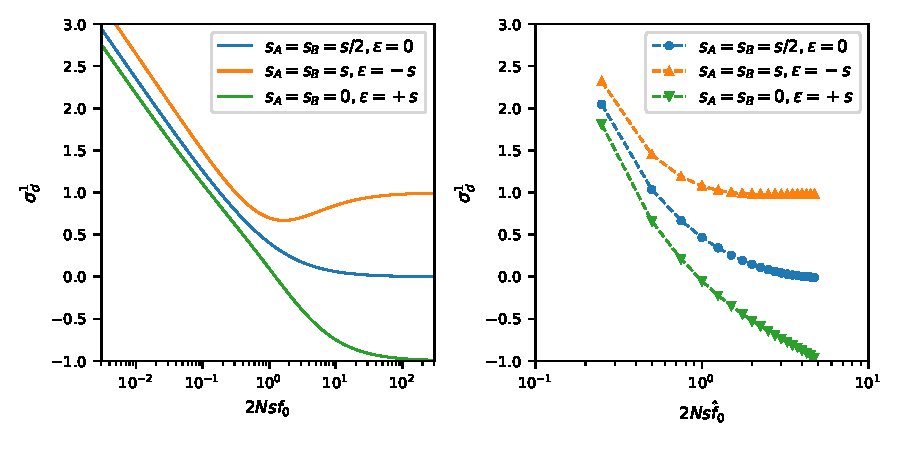
\includegraphics{./good_comparison}
    \caption{
        Left: Attempt to recreate analytical curves shown in Good (2020) Figure 3,
        using equation C9 and Scipy's \texttt{scipy.special.hyp2f1} function in Python.
        Behavior is qualitatively similar, but differs from Figure 3 in Good. 
        Right: Approximate frequency-conditioned signed LD, where
        $\hat{f}_0 = n_A/n$ and $n_B/n$, so these
        are not unbiased estimates of frequency conditioned $\sigma_d^1$ and cannot
        be compared directly.
    }
    \label{fig:good}
\end{figure}

4) I find many of the results of these simulations really intriguing: it is
notable that population expansions do not appear to change patterns of LD, and
the dominance can have such complex effects on LD (e.g Fig 2B). It would be a
valuable contribution to the literature to expand on these analyses and
describe the intuition behind these observations, though I understand it may be
beyond the scope of this study.

\begin{response}
    I have expanded the numerical and simulation results for both dominance
    and non-steady-state demography. I agree that the complex effects of
    dominance on LD are worth exploring further, especially contrasting the
    results in this paper with Roze (2021). I do think that fully diving into
    this is a bit beyond the scope of this study, but hopefully the expanded
    results and discussion on these points are still helpful.
\end{response}

5) The results on the importance of classifying mutations by the functional
annotations of the regions in which they occur is intriguing and important and
overall I think that despite these patterns being weak, they are interesting
and the section is well-caveated. However, I struggle to make a direct
connection between the intuition derived from previous part of the manuscript
and the conclusions made here. In addition to the concerns raised above to do
with comparing the results of a limited number of two-locus numerical results
to a fundamentally multi-locus system, and the specific concern about the
finding of likely epistasis between mutations within genes, I find that
statements like the one on line 313-316 require further substantiation or
should be weakened: they rely on a quantitative extrapolation that clearly
depends on the parameters and model assumptions.

\begin{response}
    I have attempted to better caveat some of these interpretations, like
    those lines that you highlight. I also now include a statement that more detailed
    modeling and comparisons in a statistical framework will be needed to
    make firm conclusions.
\end{response}


Minor comments:

1) Line 117: Although a well known quantity, it would be good to define $D$
here, since it's the first time it appears.

\begin{response}
    Thank you for the suggestion. $D$ is now defined here.
\end{response}

2) Figure 1: I suggest considering using different colors for panels C-F
compared to A-B to highlight that a different parameter is being varied in
these panels.

\begin{response}
    I have done quite a bit of figure rearrangement, careful to make color schemes
    more distinguishable.
\end{response}

3) Line 151-152: The closed form approached used here should be contrasted with
the fact that it is in principle not possible to include the effects of other
loci, unlike in these other approaches.

\begin{response}
    Thank you for the suggestion. I now point out that it not possible to include
    the effects of other linked loci above this section, when introducing the
    methods.
\end{response}

4) Figure 4: consider making the y axis consistent between panels.

\begin{response}
    There are new figures in this version of the paper, with hopefully cleaner presentation.
\end{response}

\end{document}
